\documentclass[11 pt]{article}

% Formatting
\usepackage[utf8]{inputenc}
\usepackage[margin=1in]{geometry}
\usepackage[titletoc,title]{appendix}

% Images
\usepackage{graphicx,float}

% Math
\usepackage{amsmath,amsfonts,amssymb,mathtools}

% Algorithms
\usepackage[ruled,vlined]{algorithm2e}
\usepackage{algorithmic}

% Code syntax highlighting
\usepackage{minted}
\usemintedstyle{borland}
\usepackage{listings}

% Text boxes
\usepackage{tcolorbox}

% Links
\usepackage{hyperref}

% Title content
\title{
    HW3 - Implementation of RSA \\
    \large CNS Course Sapienza
}
\author{Sultan Umarbaev, Matricola: 1954544}
\date{20/11/2020}

\begin{document}

\maketitle

% Goal
\section{Goal}
The goal of this homework is to implement RSA. It is an asymmetric cryptographic algorithm which is widely used for secure data transmission. Asymmetric cryptography is a cryptographic system that uses pairs of keys: \textit{public keys}(can be given to anyone) and \textit{private keys}(must be kept private). The generation of such keys depends on algorithms based on mathematical problems to produce one-way functions, which means that by encrypting a message with one key(e.g. public key), it can not be decrypted using the same key, the decryption is performed with the other key(e.g. private key).

% Implementation
\section{Implementation}
The programming language used for the implementation is \textit{C++}. Main library for working with large numbers is \textit{The GNU Multiple Precision Arithmetic Library} (GMP) wrapper for \textit{C++}. It is a libraray for \textbf{arbitrary-precision arithmetic} with basic interface for \textit{C} programming language and wrappers for other languages like \textit{C++}, \textit{C\#}, \textit{Python}, \textit{R}, etc. The main applications of GMP involve fields such as cryptography, Internet Security and computer algebra systems(CAS) \cite{GMP}. 
\newline
The RSA algorithm consists of four steps \cite{RSA operation wiki}:
\begin{itemize}
	\item Key generation
	\item Key distribution
	\item Encryption
	\item Decryption
\end{itemize}
\textit{Key distribution} step out of the scope of the homework.

% Implementation/Key generation
\subsection{Key generation}
The initial step in key generation process is to select 2 distinct large prime numbers \textit{p} and \textit{q}. For security purposes, \textit{p} and \textit{q} should be chosen at random and kept secret.
\newline
After choosing prime numbers, they are multiplied to give a very large number with 2 prime factors: $p * q = n$. It is used as the modulus for public and private keys. Its length in bits is the \textit{key length}. It is a part of public key.
\newline
Next step is the calculation of the \textbf{totient} of \textit{n}, which is the number of positive integers smaller than \textit{n} that are coprime to \textit{n}. For any prime number, $\phi(p)=p-1$, hence for the modulus \textit{n} with 2 prime factors $\phi(n)=(p-1)(q-1)$. It should be kept secret.
\newline
Subsequently, \textit{e} and \textit{d} are generated. Where \textit{e} is an integer that satisfies 2 conditions: $1 < e < \phi(n)$ and $gcd(e, \phi(n)) = 1$; i.e. \textit{e} and $\phi(n)$ are coprime. For more efficient encryption, \textit{e} is short bit-length and the most commonly chosen value for \textit{e} is $2^{16} + 1 = 65537$. An integer \textit{d} should satisfy the congruence relation $de \equiv 1 \pmod{\phi(n)}$, i.e. \textit{d}  is the modular multiplicative inverse of \textit{e} modulo $\phi(n)$. It must be kept secret. Public(encryption) key $(e, n)$ and private(decryption) key $(d, n)$ are generated. 
\newline
In the current implementation, prime numbers \textit{p} and \textit{q} are generated with the help of GMP library \textit{random number generation} and \textit{prime number test} functions. According to the library manual \cite{Random gen}, random number generation function used in the current implementation is based on \textbf{Mersenne Twister algorithm} and considered to be fast and have good randomness properties. The primality test consists of 2 testing algorithms \textbf{Baillie-PSW probable prime test} and \textbf{Miller-Rabin probabilistic primality tests} \cite{Prime test}.
\newline
The modular inverse of \textit{e} is calculated using the \textbf{extended Euclidean algorithm} \cite{EEA}, which is an extension to the Euclidean algorithm. In addition to the greatest common divisor (gcd) of integers \textit{a} and \textit{b}, it also computes the coefficients of \textbf{Bézout's identity}, which are integers \textbf{x} and \textbf{y}:
\begin{equation}
    ax+by=\gcd(a,b)
\end{equation}
In the case of RSA, the equation looks like this:
\begin{equation}
    ed+\phi(n)y=\gcd(e, \phi(n))=1
\end{equation}
Then, if $\mod \phi(n)$ is taken of both sides, the $\phi(n)y$ disappears, and the equation becomes:
\begin{equation}
    ed \equiv 1 \mod \phi(n)
\end{equation}
Hence, coefficient \textit{x} of \textbf{Bézout's identity} is the multiplicative inverse of the \textit{e} (\textit{d} generation function in Figure~\ref{fig:multiplicative-inverse-calculation} in Appendix~\ref{appendix:source-code-functions}).

% Implementation/Encryption and Decryption
\subsection{Encryption and Decryption}
Public key $(e, n)$ is released by one person and anyone with it can encrypt message. Message \textit{M} is turned into an integer \textit{m} such that $0 \leq m < n$ and ciphertext \textit{c} is computed corresponding to: $m^{e} \equiv c \pmod{n}$. Ciphertext \textit{c} is then sent to the one who generated public key.
\newline
Decryption is performed using private key $(d,n)$ given ciphertext \textit{c}: $c^{d}\equiv (m^{e})^{d}\equiv m{\pmod {n}}$, hence recovering the original message \textit{M}.
\newline
Since \textit{m} and \textit{n} are large numbers, the performance of exponentiation operation is slow. It can be resolved using modular exponentiation. \textbf{Right-to-left binary method} \cite{Right-to-left binary method} is a combination of the \textbf{Binary Exponentiation algorithm} and modulo arithmetic. It is memory-efficient and reduces the number of operations to perform modular exponentiation. The idea of binary exponentiation is to use the binary representation of the exponent, Equation~\ref{eqn:e-converted-to-binary-notation}.
\begin{equation}
e=\sum _{i=0}^{n-1}a_{i}2^{i}
\label{eqn:e-converted-to-binary-notation}
\end{equation}
Where $a_{i}$ can be 0 or 1. As a result, $b^e$ can be rewritten to Equation~\ref{eqn:b-to-the-power-of-e}.
\begin{equation}
b^{e}=b^{\left(\sum _{i=0}^{n-1}a_{i}2^{i}\right)}=\prod _{i=0}^{n-1}b^{a_{i}2^{i}}
\label{eqn:b-to-the-power-of-e}
\end{equation}
For example, $b^{13}=b^{1101_{2}}=b^{1*2^3}⋅b^{1*2^2}⋅b^{0*2^2}⋅b^{1*2^1}=b^{8}⋅b^{4}⋅b^{0}⋅b^{1}$. Since the modulo operator doesn't interfere with multiplications: $a⋅b \equiv (a \mod m)⋅(b \mod m) \mod m$, therefore:
\begin{equation}
c \equiv \prod _{i=0}^{n-1}b^{a_{i}2^{i}}{\pmod {m}}
\label{eqn:modulo-exponentiation}
\end{equation}

\begin{algorithm}
    \begin{algorithmic}
        \STATE{$result\gets 1$}
        \STATE{$base\gets base \mod modulus$}
        \WHILE{$exponent > 0$}
            \IF{$exponent \mod 2 == 1$}
                \STATE{$result\gets (result*base) \mod modulus$}
            \ENDIF
            \STATE{$exponent\gets exponent >> 1$}
            \STATE{$base\gets (base*base) \mod modulus$}
        \ENDWHILE
        \RETURN result
    \end{algorithmic}
\caption{Right-to-left binary algorithm pseudocode \cite{Right-to-left binary method}}
\label{alg:right-to-left-binary-algorithm}
\end{algorithm}
\newline
The running time of this algorithm is O($log_{2}$ \textit{exponent}), while time of naive approach is O(\textit{exponent}). For instance, consider $exponent=4294967296$, this algorithm would require 32 ($2^{32} = 4294967296$) steps to perform an exponentiation instead of 4294967296 steps \cite{Right-to-left binary method}.
\newline
The exponentiation operation for encryption and decryption processes of the current implementation of RSA utilizes the described algorithm (see Figure~\ref{fig:modular-exponentiation-calculation} in Appendix~\ref{appendix:source-code-functions}).

% Implementation/Limitations and weaknesses
\subsection{Limitations and weaknesses}
The main weakness of the current implementation is the absence of \textbf{Padding Scheme}. The absence of padding makes RSA vulnerable to the number of attacks \cite{RSA padding wiki, Asymmetric Ciphers II} considering different cases: 
\begin{itemize}
	\item size of the message and exponent are too small
	\item same message is encrypted using same exponent, but with different modulus
	\item same message is encrypted using coprime exponent, but with same modulus
\end{itemize}
In addition, RSA without padding is not \textbf{semantically secure} which means that information about the message can be feasibly extracted from the ciphertext. This allows an attacker to perform \textbf{chosen-ciphertext attack} \cite{RSA padding wiki}.
\newline
Practical and real-world RSA implementations are built with padding schemes. Randomized padding is added into the message before encrypting it resulting in less predictable message structure. It must be carefully designed to avoid and prevent mentioned attacks \cite{RSA padding wiki}.

% Results
\section{Results} 
The current implementation of RSA is capable of performing 3 out 4 steps of RSA algorithm: key generation, encryption and decryption. \textit{Key generation} operation can generate keys of size up to 4096 bit-length. However, it does not provide \textit{key management}, as a result keys are stored in raw format as a plaintext, Figure~\ref{fig:public-and-private-keys}. Public key consists of key size, \textit{e}, \textit{n}, Key size is embedded in public key to avoid situation where data size $>$  \textit{n}. Private key involves \textit{d} and \textit{n}.
\begin{figure}[H]
    \centering
    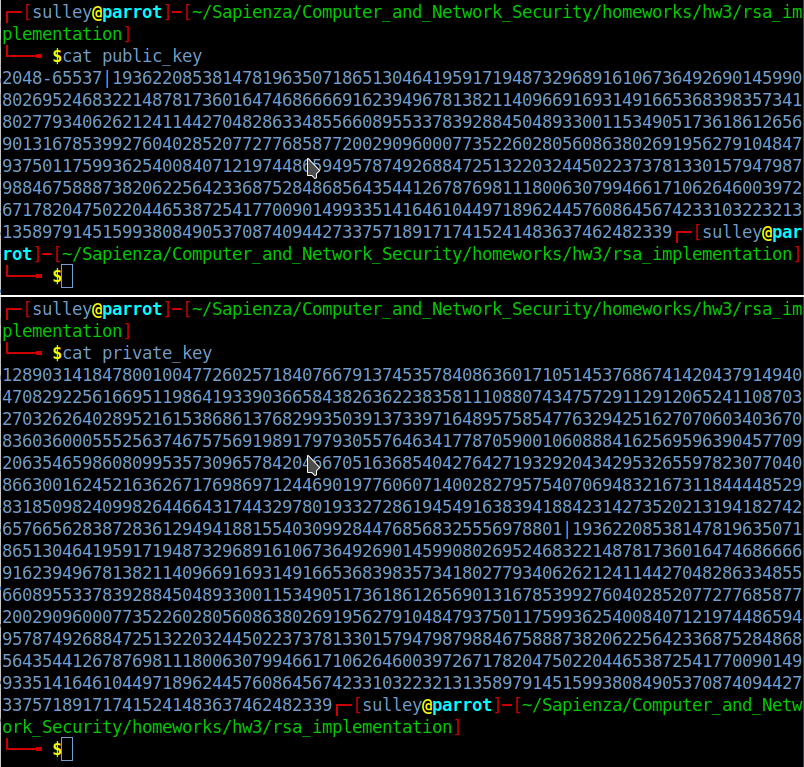
\includegraphics[width=1\linewidth]{rsa_implementation_keys.png}
    \caption{Public and private keys of RSA implementation.}
    \label{fig:public-and-private-keys}
\end{figure}

The encrypted message is not encoded and stored as a big number in the file, see Figure~\ref{fig:rsa-implementation-encrypted-data}. The size of the encrypted message depends on the size of the key, \textit{n}, thus the message size has to be $n/8$ bytes size, considering the absence of padding. However it was detected and noted that the \textit{encryption} and \textit{decryption} operations of the current implementation can only work with the sizes slightly lower than expected ones. For instance:
\begin{itemize}
	\item with the key size 4096 bits, the message size has to be less than 512 bytes, and current implementation can not properly encrypt and decrypt data more than 410 bytes.
	\item with the key size 2048 bits, the requirement is $m<256$ bytes, however the actual threshold is approximately 200.
\end{itemize}
This issue hasn't been resolved yet and is on the list of tasks, alongside with padding scheme and encrypted message encoding, for the future improvements.

\begin{figure}[H]
    \centering
    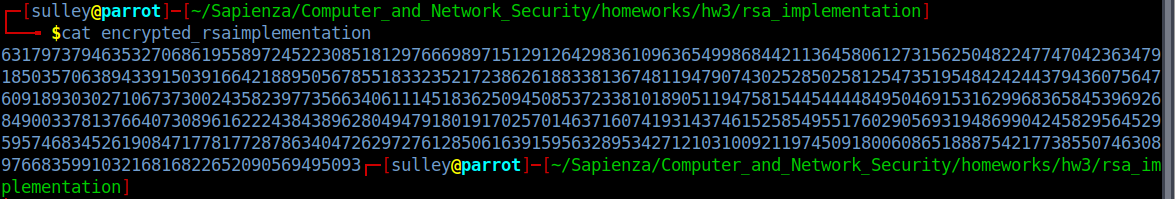
\includegraphics[width=1\linewidth]{rsa_implementation_encrypted_data.png}
    \caption{Encrypted data of RSA implementation.}
    \label{fig:rsa-implementation-encrypted-data}
\end{figure}
\newline

% Experimental comparison
\section{Experimental comparison}
Considering the comparison, it was experimented with OpenSSL implementations of RSA and AES. The experiment consists of encryption and decryption performance speed, see Figures~\ref{fig:openssl-aes-speed},~\ref{fig:openssl-rsa-speed},~\ref{fig:rsa-implementation-speed}. The file size for experiment is 199 bytes. The key size is chosen to be 2048 bits long. Based on the results, it can be concluded that the speed of encryption process is approximately identical, if not. However, the decryption speed ranks them in the following order: OpenSSL AES-256 with 0.002 seconds, OpenSSL RSA with 0.003 seconds, RSA implementation with 0.006 seconds.

\begin{figure}[H]
    \centering
    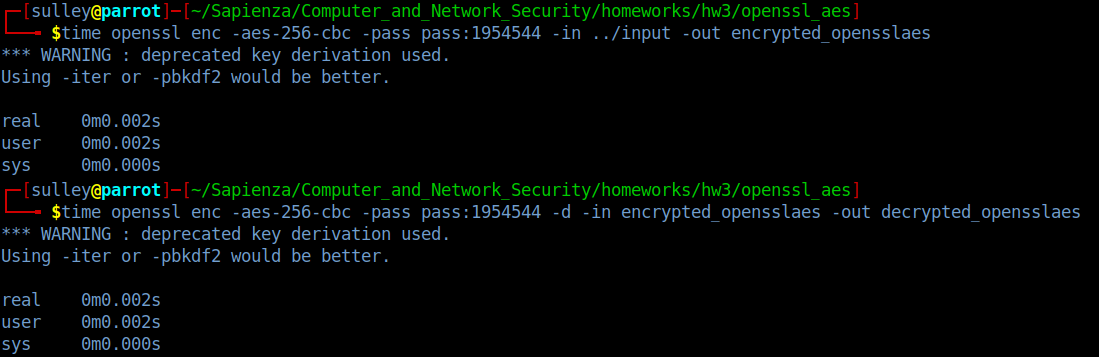
\includegraphics[width=1\linewidth]{openssl_aes_speed_results.png}
    \caption{OpenSSL AES-256 encryption and decryption speed results.}
    \label{fig:openssl-aes-speed}
\end{figure}

\begin{figure}[H]
    \centering
    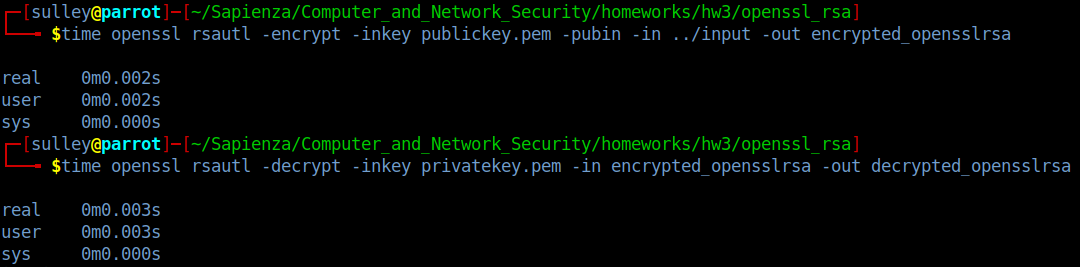
\includegraphics[width=1\linewidth]{openssl_rsa_speed_results.png}
    \caption{OpenSSL RSA encryption and decryption speed results.}
    \label{fig:openssl-rsa-speed}
\end{figure}

\begin{figure}[H]
    \centering
    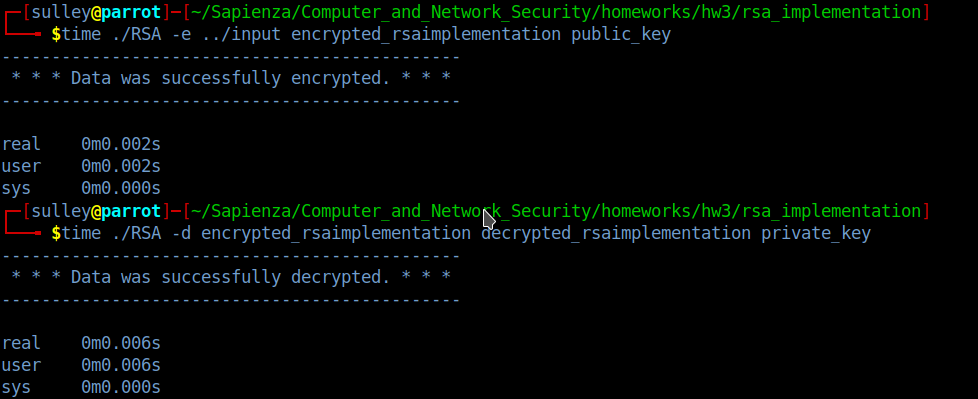
\includegraphics[width=1\linewidth]{rsa_implementation_speed_results.png}
    \caption{RSA implementation encryption and decryption speed results.}
    \label{fig:rsa-implementation-speed}
\end{figure}

\newline
In addition, the performance speed of \textit{key generation} step of RSA implementations were compared, see Figures~\ref{fig:openssl-rsa-keygen-speed},~\ref{fig:rsa-implementation-keygen-speed}. The speed results of the RSA implementation seem to be better, however it is all due to the absence of \textit{key management} process. 

\begin{figure}[H]
    \centering
    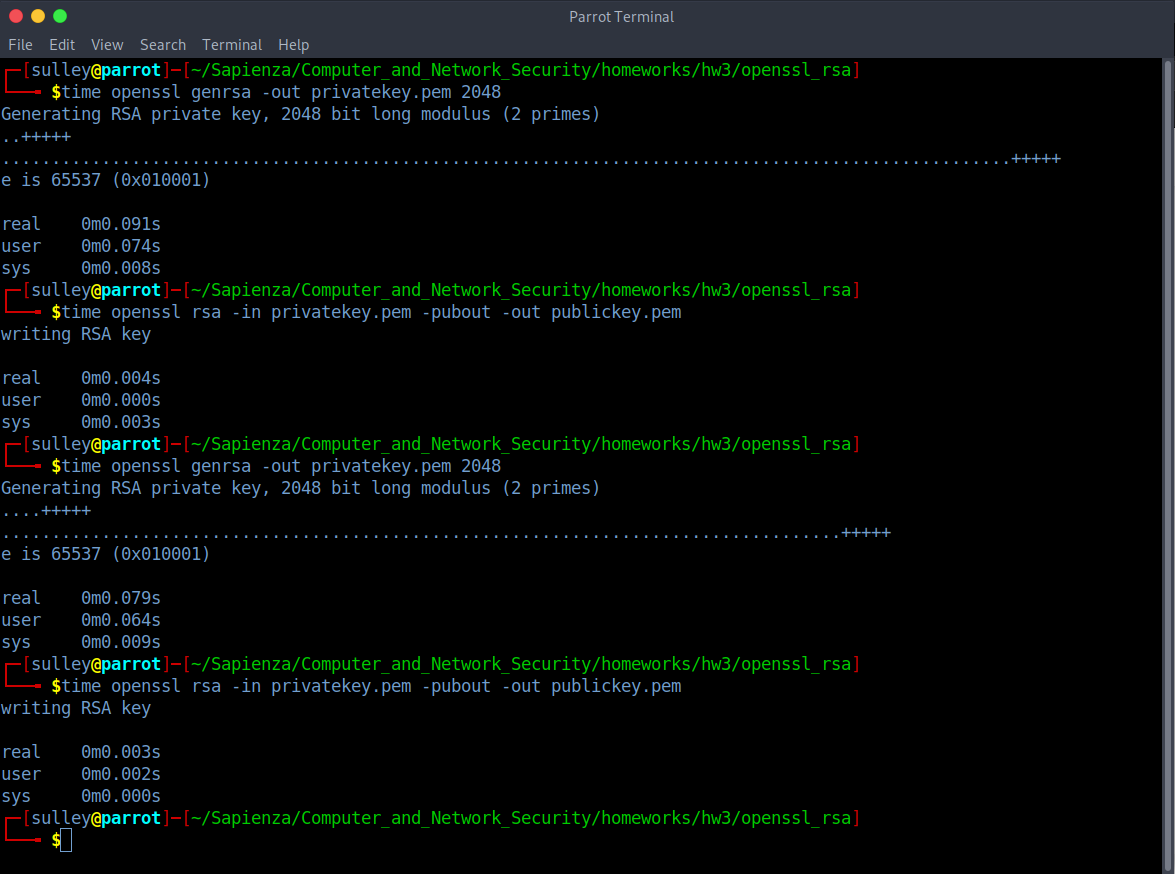
\includegraphics[width=0.9\linewidth]{openssl_rsa_keygen_speed.png}
    \caption{OpenSSL RSA key generation speed results.}
    \label{fig:openssl-rsa-keygen-speed}
\end{figure}

\begin{figure}[H]
    \centering
    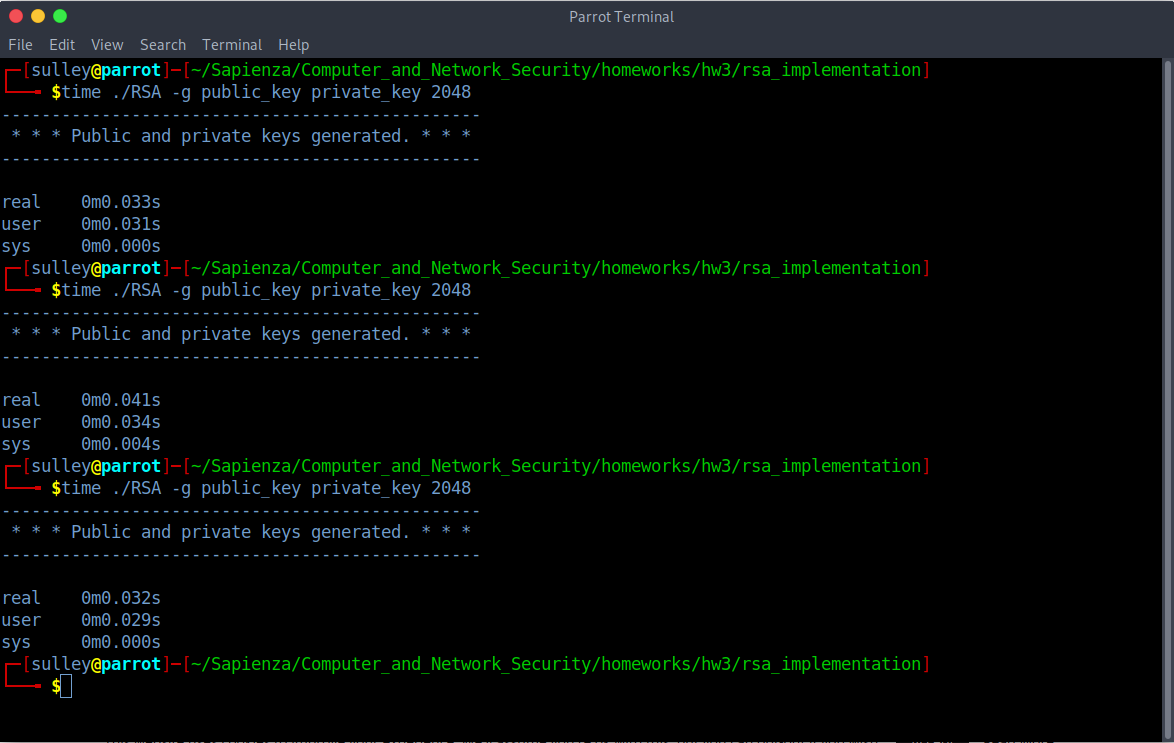
\includegraphics[width=0.9\linewidth]{rsa_implementation_keygen_speed.png}
    \caption{RSA implementation key generation speed results.}
    \label{fig:rsa-implementation-keygen-speed}
\end{figure}

% Conclusion
\section{Conclusion}
The goal of implementing RSA algorithm was achieved, however it requires improvements and is not recommended for practical use. RSA is a relatively slow algorithm and is not practical to use with large data comparing to AES. As a result, it is not commonly used for user data encryption and decryption. Practically, RSA is used to transmit shared keys for symmetric key cryptography, which are then used to encrypt and/or decrypt data. 

% References
\begin{thebibliography}{10}

    \bibitem{GMP}
	GNU Multiple Precision Arithmetic Library, URL: \url{https://en.wikipedia.org/wiki/GNU_Multiple_Precision_Arithmetic_Library}
	
    \bibitem{RSA operation wiki}
	RSA (cryptosystem) operation, URL: \url{https://en.wikipedia.org/wiki/RSA_(cryptosystem)#Operation}

    \bibitem{Random gen}
	Random State Initialization, URL: \url{https://gmplib.org/manual/Random-State-Initialization#Random-State-Initialization}

    \bibitem{Prime test}
	Number Theoretic Functions, URL: \url{https://gmplib.org/manual/Number-Theoretic-Functions}

    \bibitem{EEA}
	Modular multiplicative inverse, URL: \url{https://en.wikipedia.org/wiki/Modular_multiplicative_inverse#Extended_Euclidean_algorithm}

	\bibitem{Right-to-left binary method}
	Right-to-left binary method, URL: \url{https://en.wikipedia.org/wiki/Modular_exponentiation#Right-to-left_binary_method}
	
	\bibitem{RSA padding wiki}
	RSA (cryptosystem) padding wiki, URL: \url{https://en.wikipedia.org/wiki/RSA_(cryptosystem)#Padding}

	\bibitem{Asymmetric Ciphers II}
	Asymmetric Ciphers II, URL: \url{https://piazza.com/class_profile/get_resource/kf2apkmqhrq4qw/kgrqkx1l5wt3ux}
	
\end{thebibliography}

% Appendices
\begin{appendices}

% Screenshots
\section{Functions from source code}
\begin{figure}[H]
    \centering
    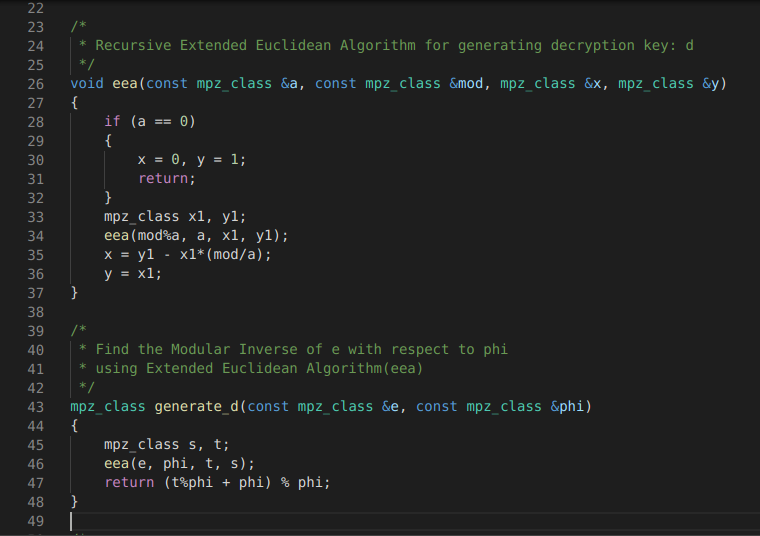
\includegraphics[width=1\linewidth]{multiplicative_inverse_calculation.png}
    \caption{Multiplicative inverse calculation.}
    \label{fig:multiplicative-inverse-calculation}
\end{figure}
\begin{figure}[H]
    \centering
    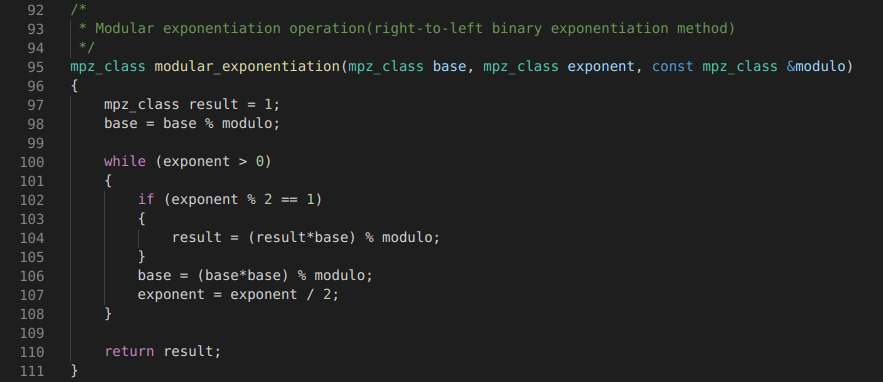
\includegraphics[width=1\linewidth]{modular_exponentiation_calculation.png}
    \caption{Modular exponentiation calculation.}
    \label{fig:modular-exponentiation-calculation}
\end{figure}
\label{appendix:source-code-functions}

\end{appendices}

\end{document}
